%%%%%%%%%%%%%%%%%%%%%%%%%%%%%%%%%%%%%%%%%
% Journal Article
% LaTeX Template
% Version 1.3 (9/9/13)
%
% This template has been downloaded from:
% http://www.LaTeXTemplates.com
%
% Original author:
% Frits Wenneker (http://www.howtotex.com)
%
% License:
% CC BY-NC-SA 3.0 (http://creativecommons.org/licenses/by-nc-sa/3.0/)
%
%%%%%%%%%%%%%%%%%%%%%%%%%%%%%%%%%%%%%%%%%

%----------------------------------------------------------------------------------------
%	PACKAGES AND OTHER DOCUMENT CONFIGURATIONS
%----------------------------------------------------------------------------------------

\documentclass[twoside]{article}

\usepackage{biblatex}
\bibliography{project.bib}

\usepackage[sc]{mathpazo} % Use the Palatino font
\usepackage[T1]{fontenc} % Use 8-bit encoding that has 256 glyphs
\usepackage[utf8]{inputenc}
\linespread{1.05} % Line spacing - Palatino needs more space between lines
\usepackage{microtype} % Slightly tweak font spacing for aesthetics

\usepackage[hmarginratio=1:1,top=32mm,columnsep=20pt]{geometry} % Document margins
\usepackage{multicol} % Used for the two-column layout of the document
\usepackage[hang, small,labelfont=bf,up,textfont=it,up]{caption} % Custom captions under/above floats in tables or figures
\usepackage{booktabs} % Horizontal rules in tables
\usepackage{float} % Required for tables and figures in the multi-column environment - they need to be placed in specific locations with the [H] (e.g. \begin{table}[H])
\usepackage{hyperref} % For hyperlinks in the PDF

\usepackage{lettrine} % The lettrine is the first enlarged letter at the beginning of the text
\usepackage{paralist} % Used for the compactitem environment which makes bullet points with less space between them

\usepackage{listings}
   \usepackage[pdftex]{graphicx} 

\usepackage{abstract} % Allows abstract customization
\renewcommand{\abstractnamefont}{\normalfont\bfseries} % Set the "Abstract" text to bold
\renewcommand{\abstracttextfont}{\normalfont\small\itshape} % Set the abstract itself to small italic text

\usepackage{titlesec} % Allows customization of titles
\renewcommand\thesection{\Roman{section}} % Roman numerals for the sections
\renewcommand\thesubsection{\Roman{subsection}} % Roman numerals for subsections
\titleformat{\section}[block]{\large\scshape\centering}{\thesection.}{1em}{} % Change the look of the section titles
\titleformat{\subsection}[block]{\large}{\thesubsection.}{1em}{} % Change the look of the section titles

\usepackage{fancyhdr} % Headers and footers
\pagestyle{fancy} % All pages have headers and footers
\fancyhead{} % Blank out the default header
\fancyfoot{} % Blank out the default footer
\fancyhead[C]{LINGI2141 - Individual Project $\bullet$ December 2013 } % Custom header text
\fancyfoot[RO,LE]{\thepage} % Custom footer text

%----------------------------------------------------------------------------------------
%	TITLE SECTION
%----------------------------------------------------------------------------------------

\title{\vspace{-15mm}\fontsize{24pt}{10pt}\selectfont\textbf{LINGI2141 - Individual Project \\Analysis of APT-GET}} % Article title

\author{
\large
\textsc{Benoît Baufays}\\[2mm] % Your name
\normalsize Université Catholique de Louvain \\ % Your institution
\vspace{-5mm}
}
\date{}

%----------------------------------------------------------------------------------------

\begin{document}

\maketitle % Insert title

\thispagestyle{fancy} % All pages have headers and footers

%----------------------------------------------------------------------------------------
%	ABSTRACT
%----------------------------------------------------------------------------------------

\begin{abstract}

This paper will deal with analysing the managing software apt-get wich are deployed on several linux distributions 

\end{abstract}

%----------------------------------------------------------------------------------------
%	ARTICLE CONTENTS
%----------------------------------------------------------------------------------------

\begin{multicols}{2} % Two-column layout throughout the main article text

\section{Introduction}

\lettrine[nindent=0em,lines=3]{A} pt-get is a software develloped for linux OS to centralize the management of your software.  Apt-get install packages  containing precompiled code, configuration files, and meta-information about the package.  Because it is not very usefull to manage manually all your packages, apt-get was created.  With him, you can update your system and yours packages but you can also install or remove packages.  The utility of apt-get is the management of the dependencies and, with one program, you can maintain your system up to date.

\section{Apt-get}
Apt-get have several commands, depending on what you want to do.
\begin{itemize}
	\item update : with this command, apt-get search, on remotes servers, the last version for all packets.  It get also the entire list of packets you can install via apt-get;
	\item upgrade or dist-upgrade : with this command, apt-get downloads packets installed on your system wich are to be updated.  The difference between the command "upgrade" and "dist-upgrade" is that, whit hthe first, apt-get doesn't install new packages.  For example, some packages must requires new dependencies.  If you update with the first command, apt-get doesn't install new dependencies and, of course, doesn't update the packet.  In other hand, with the second command, apt-get install all dependencies and update all packages;
	\item install : with this command, you can install new package.  Apt-get search for dependencies and install the package and the required packages;
	\item remove : with this command, apt-get remove the package mentionned.  It can also remove packages wich are not still required on your system.  For example, if a package is only installed because it is a dependency for an other package and you remove this package, it is not require to have the dependency's package on your system.
\end{itemize}
Apt-get have several others command but the main has be presented below.  To analyse how apt-get works and deal with network, we will use the same order presented in the list below.  But, before, we discuss about the IPv 6 and apt-get.

\section{Apt-get and IPv6}
To know where it must searching informations about packages, apt-get have one file "/etc/apt/sources.list" which contains addresses of servers.  According to several bloggers, apt-get have some troubles with IPv6 because some servers have no Ipv6 address or the ISP doesn't support it.\\
To verify this information, we have used dig to send a DNS request to archive.ubuntu.com, the main server for every sources.\\ \\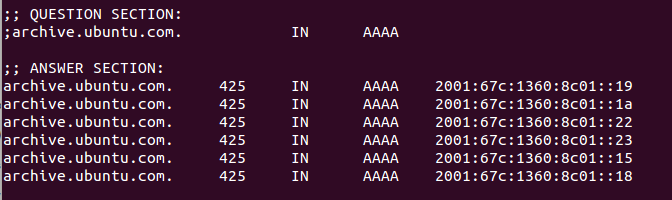
\includegraphics[scale=0.3]{pictures/DNS_info.png}



As we can see, archive.ubuntu.com have several IPv6 address, the problem do not come form that.  When we go deeper in the code of apt-get, we see that some functionnalities are still using IPv4 libraries.

\section{Apt-get analysis}
\subsection{Update}
\subsubsection{DNS Request}
With this command, apt-get read first the file containing all server's name.  With this information, it sends DNS request to know IP address of each server. \\ \\ 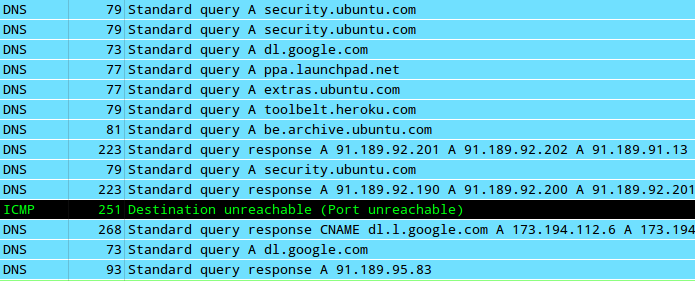
\includegraphics[scale=0.32]{pictures/dns_update.png}

As we can see, Apt-get send first all his DNS requests before contacting servers.  We see also that dl.google.com, an entry that we have added manually to access to packages from Google (GoogleTalk, ...) is, in reality, reachable via dl.l.google.com.  Finally, we can see that apt-get send twice the DNS request about dl.google.com.  It's not beacause it doesn't receive the response but because we have added twice this entry in the config file.\\
To test the DNS system, we have put manually a arbitrary IP address for the second DNS server.  This test is visible in the schema below with the "Destination unreachable" message.  After that, apt-get doesn't reuse this IP adress to send DNS query.\\
When we analysing packets receive by apt-get, we see that the time life of the information is 3 minutes 30.  Also, we see that it receive more than one IP address for every server name.  With this solution, apt-get doesn't want  to resend a DNS query if a IP adress down.  With multiple IP adresses, it can also  use multi threading and request informations on multiple servers.\\
\subsubsection{Getting information}
With the IP address, apt-get can now getting informations about packages.  These informations are getting in two step.\\ \\ 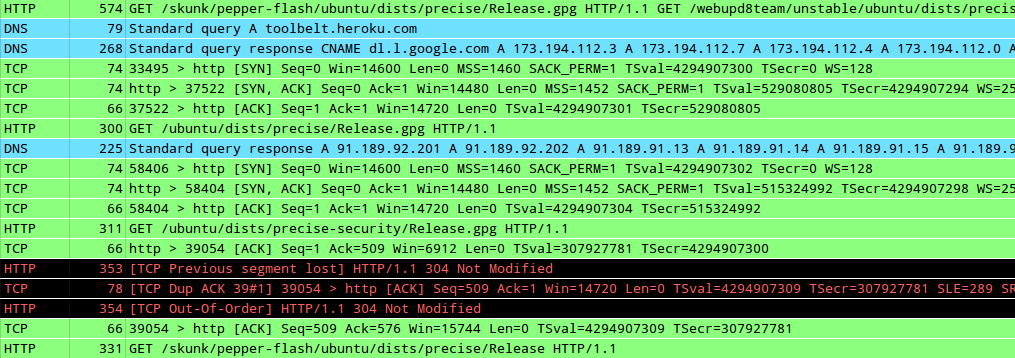
\includegraphics[scale=0.2]{pictures/update_get_1.png}

%------------------------------------------------

%------------------------------------------------

%------------------------------------------------


%----------------------------------------------------------------------------------------
%	REFERENCE LIST
%----------------------------------------------------------------------------------------

\printbibliography

%----------------------------------------------------------------------------------------

\end{multicols}

\end{document}
